\PassOptionsToPackage{unicode=true}{hyperref} % options for packages loaded elsewhere
\PassOptionsToPackage{hyphens}{url}
\documentclass[11pt,dvipsnames,ignorenonframetext,aspectratio=169]{beamer}
\IfFileExists{pgfpages.sty}{\usepackage{pgfpages}}{}
\setbeamertemplate{caption}[numbered]
\setbeamertemplate{caption label separator}{: }
\setbeamercolor{caption name}{fg=normal text.fg}
\beamertemplatenavigationsymbolsempty
\usepackage{lmodern}
\usepackage{amssymb,amsmath}
\usepackage{ifxetex,ifluatex}
\usepackage{fixltx2e} % provides \textsubscript
\ifnum 0\ifxetex 1\fi\ifluatex 1\fi=0 % if pdftex
  \usepackage[T1]{fontenc}
  \usepackage[utf8]{inputenc}
\else % if luatex or xelatex
  \ifxetex
    \usepackage{mathspec}
  \else
    \usepackage{fontspec}
\fi
\defaultfontfeatures{Ligatures=TeX,Scale=MatchLowercase}







\fi

  \usetheme[]{monash}

  \usecolortheme{monashwhite}


% A default size of 24 is set in beamerthememonash.sty

% Title page
\setbeamertemplate{title page}
{\placefig{-0.01}{-0.01}{width=1.01\paperwidth,height=1.01\paperheight}{white\_rose.jpg}
\begin{textblock}{7.5}(1,2.8)\usebeamerfont{title}
{\color{white}\raggedright\par\inserttitle}
\end{textblock}
\begin{textblock}{7.5}(1,7)
{\color{white}\raggedright{\insertauthor}\mbox{}\\[0.2cm]
\insertdate}
\end{textblock}}


  \useinnertheme{rounded}

  \useoutertheme{smoothtree}

% use upquote if available, for straight quotes in verbatim environments
\IfFileExists{upquote.sty}{\usepackage{upquote}}{}
% use microtype if available
\IfFileExists{microtype.sty}{%
  \usepackage{microtype}
  \UseMicrotypeSet[protrusion]{basicmath} % disable protrusion for tt fonts
}{}


\newif\ifbibliography
  \usepackage[round]{natbib}
  \bibliographystyle{plainnat}


\hypersetup{
      pdftitle={Development of Resistant Varieties in Nepal},
            colorlinks=true,
    linkcolor=red,
    citecolor=Blue,
    urlcolor=pink,
    breaklinks=true}
%\urlstyle{same}  % Use monospace font for urls







% Prevent slide breaks in the middle of a paragraph:
\widowpenalties 1 10000
\raggedbottom

  \AtBeginPart{
    \let\insertpartnumber\relax
    \let\partname\relax
    \frame{\partpage}
  }
  \AtBeginSection{
    \ifbibliography
    \else
      \let\insertsectionnumber\relax
      \let\sectionname\relax
      \frame{\sectionpage}
    \fi
  }
  \AtBeginSubsection{
    \let\insertsubsectionnumber\relax
    \let\subsectionname\relax
    \frame{\subsectionpage}
  }



\setlength{\parindent}{0pt}
\setlength{\parskip}{6pt plus 2pt minus 1pt}
\setlength{\emergencystretch}{3em}  % prevent overfull lines
\providecommand{\tightlist}{%
  \setlength{\itemsep}{0pt}\setlength{\parskip}{0pt}}

  \setcounter{secnumdepth}{0}


%% Monash overrides
\AtBeginSection[]{
   \frame<beamer>{
   \frametitle{Outline}\vspace*{0.2cm}
   
   \tableofcontents[currentsection,hideallsubsections]
  }}

% Redefine shaded environment if it exists (to ensure text is black)
\ifcsname Shaded\endcsname
  \definecolor{shadecolor}{RGB}{225,225,225}
  \renewenvironment{Shaded}{\color{black}\begin{snugshade}\color{black}}{\end{snugshade}}
\fi
%%


  \usepackage{setspace}
  \usepackage{wasysym}
  % \usepackage{footnote} % don't use this this breaks all
  \usepackage{fontenc}
  \usepackage{fontawesome}
  \usepackage{booktabs,siunitx}
  \usepackage{longtable}
  \usepackage{array}
  \usepackage{multirow}
  \usepackage{wrapfig}
  \usepackage{float}
  \usepackage{colortbl}
  \usepackage{pdflscape}
  \usepackage{tabu}
  \usepackage{threeparttable}
  \usepackage{threeparttablex}
  \usepackage[normalem]{ulem}
  \usepackage{makecell}
  \usepackage{xcolor}
  \usepackage{tikz} % required for image opacity change
  \usepackage[absolute,overlay]{textpos} % for text formatting
  \usepackage{chemfig}
  \usepackage[skip=0.333\baselineskip]{caption}
  % \newcommand*{\AlignChar}[1]{\makebox[1ex][c]{\ensuremath{\scriptstyle#1}}}%
  \usepackage{siunitx}

  % this font option is amenable for beamer
  \setbeamerfont{caption}{size=\tiny}
  \singlespacing
  \definecolor{lightgrayd}{gray}{0.95}
  \definecolor{skyblued}{rgb}{0.65, 0.6, 0.94}
  \definecolor{oranged}{RGB}{245, 145, 200}

  % % better to insert it into template itself
  % \newlength{\cslhangindent}
  % \setlength{\cslhangindent}{1.5em}
  % \newenvironment{cslreferences}%
  %   {\setlength{\parindent}{0pt}%
  %   \everypar{\setlength{\hangindent}{\cslhangindent}}\ignorespaces}%
  %   {\par}

  \usepackage[caption=false]{subfig}

  \newcommand{\bcolumns}{\begin{columns}[T, onlytextwidth]}
  \newcommand{\ecolumns}{\end{columns}}

  \newcommand{\bdescription}{\begin{description}}
  \newcommand{\edescription}{\end{description}}

  \newcommand{\bitemize}{\begin{itemize}}
  \newcommand{\eitemize}{\end{itemize}}
  \AtBeginSubsection{}

  \title[]{Development of Resistant Varieties in Nepal}


  \author[
        Deependra Dhakal\\
Assistant Professor\\
Agriculture and Forestry University\\
\textit{ddhakal.rookie@gmail.com}\\
\url{https://rookie.rbind.io}
    ]{Deependra Dhakal\\
Assistant Professor\\
Agriculture and Forestry University\\
\textit{ddhakal.rookie@gmail.com}\\
\url{https://rookie.rbind.io}}


\date[
      
  ]{
    }

\begin{document}

% Hide progress bar and footline on titlepage
  \begin{frame}[plain]
  \titlepage
  \end{frame}


   \frame<beamer>{
   \frametitle{Outline}\vspace*{0.2cm}
   
   \tableofcontents[hideallsubsections]
  }

\hypertarget{development-of-resistant-varieties}{%
\section{Development of resistant
varieties}\label{development-of-resistant-varieties}}

\begin{frame}{}
\protect\hypertarget{section}{}
\small

\begin{itemize}
\tightlist
\item
  Recently (with amendments) Seed act, 2045; National seed policy, 2056;
  Seed regulation, 2069; National seed vision, 2013-2025 have paved
  forward a way for use and distribution of varieties in Nepal.

  \begin{itemize}
  \tightlist
  \item
    In attempts to promote use of quick generated/exotic/landraces
    varieties, regulations allow \alert{registration} alongside
    \alert{release}.
  \end{itemize}
\item
  Respective commodity research programs have primarily been responsible
  for development and improvement of varieties in the past, whereas
  private sector and I/NGOs also can lead the variety maintenance and
  development works of their own.
\end{itemize}
\end{frame}

\begin{frame}{}
\protect\hypertarget{section-1}{}
\small

\begin{itemize}
\tightlist
\item
  Most breeding efforts for building resistance in crop varieties of
  Nepal are aimed at improving population level resistance to specific
  pathogen and their races.
\item
  In rice breeding, for example, selection methods have been modified to
  accomodate involvement of farming community to generate an
  \emph{improved variety}. Most commonly employed methods include:

  \begin{itemize}
  \footnotesize
  \item Modified bulk selection
  \item Stratified mass selection
  \end{itemize}
\item
  Aside from developing completely new varieties, adjustment of cropping
  practices to suit performance of existing varieties are of focus.

  \begin{itemize}
  \tightlist
  \item
    Integrated use of fungicide (e.g., fungicide spray for foliar fungal
    disease and seed treatment for seed-borne fungal disease) and
    cultivation practice (clean cultivation, solarization, residue
    burning) are practiced
  \end{itemize}
\end{itemize}

\footnotesize Note: For a tabulation of resistant varieties of all crop
categories developed in Nepal, refer to Lecture slides on ``Source and
Test of Resistance''.
\end{frame}

\hypertarget{cereal-crops}{%
\section{Cereal Crops}\label{cereal-crops}}

\begin{frame}{Breeding for rice blast resistance}
\protect\hypertarget{breeding-for-rice-blast-resistance}{}
\begin{itemize}
\tightlist
\item
  Breeding for durable blast (caused by \emph{Magnaporthe grisea}
  (Herbert) Borr.) resistance in rice requires multiple resistance genes
  to be combined into individual varieties with use of efficient
  selection and breeding strategies.
\item
  Two types of rice blast resistance has been described -- complete
  (true or vertical) and field resistance (horizontal)
  \citep{fukuoka2019strategies}.

  \begin{itemize}
  \tightlist
  \item
    breakdown of the resistance conferred by R-genes occurs every 1-7
    years after their release due to emergence of new race of blast
    pathogen.
  \end{itemize}
\item
  Inheritance is of either types -- monogenic dominant (most common),
  monogenic recessive, two dominant independent genes, two dominant
  complementary genes and two recessive duplicate genes or resistance
  controlled by minor genes
\item
  Resistance to infection by this fungus follows a classic gene for gene
  theory; \emph{Pi-b} and \emph{Pi-ta} are two major blast resistance
  genes.
\end{itemize}
\end{frame}

\begin{frame}{}
\protect\hypertarget{section-2}{}
\footnotesize

\begin{itemize}
\tightlist
\item
  Every year NARC screens more than 1000 rice genotypes using
  conventional breeding approach and more than 50\% are found to bear
  some form of resistance to blast
  fungus\footnote[frame]{\scriptsize Positive correlation between leaf and neck blast incidence are reported, hence necessiting breeding for broad spectrum resistance}.
\item
  Most of the screening germplasm are breeding lines generated from
  national commodity research programs and those received from IRRI.
\item
  International germplasm are ideal sources for introgression of new
  resistance genes in the varieties under cultivation.
\item
  Screening sites distinguished based on a broad agro-ecology and
  potential disease hotspots,

  \begin{itemize}
  \footnotesize
  \item Hid hill: Khumaltar, Lumle
  \item Terai: Hardinath
  \item Blast hot-spot: Bijayanagar (Jumla), Gokarna (Lalitpur), Chaling (Lalitpur), Dharmasthali (Kathmandu), Kavresthali (Kathmandu), Bhawasi (Mahottari)\footnote[frame]{\scriptsize A hotspot location for neck blast screening} and Bharatpur (Dhanusha).
  \end{itemize}
\item
  Laxmi, Sabitri, Janaki, Radha-12, Khumal-11 are some rice varieties
  found resistant to blast. Laxmi is resistant to the most virulent
  isolate ever tested (particular isolate could produce disease on rice
  genotype with 3 gene pyramid).
\item
  Masuli or Sankharika have shown susceptible response when tested over
  several parts of Nepal.
\item
  For screening purposes, CO39 and LTH may be regarded as susceptible
  lines and Tetap as resistant line, of cross-national origin.
\end{itemize}
\end{frame}

\begin{frame}{}
\protect\hypertarget{section-3}{}
\bcolumns
\column{0.6\textwidth}
\footnotesize

\begin{itemize}
\tightlist
\item
  Pedigree analysis of Nepalese rice cultivars indicate that 14
  ancestors of these cultivars are resistant to blast (Table
  tab:pedigree-rice-nepal)
  \footnote[frame]{\scriptsize Refer to (and transcribe, as assignment to students) the Table 2 of article by \cite{joshi2014molecular}; Link: \url{https://www.nepjol.info/index.php/AEJ/article/view/19831/16313}}
  fungus. The ancestor, Sigadis was used in deveopment of 13 cultivars.
  Because the genetic backgrounds of most modern day rice cultivars is
  rather narrow, due to being derived from a limited set of parent
  germplasm, characterization of resistance genes in various sources of
  germplasm is critical for a durable fight against blast disease.\\
\item
  Introduction of exotic germplasm in breeding programs has led to
  resurgence/outbreak of previously minor races of blast fungus,
  therefore focus should be shifted towards building durable resistance
  from the use of locally adapted germplasm with native resistance.
  Marker assisted selection should definitely prove to be a valuable
  aid.
\end{itemize}

\column{0.4\textwidth}

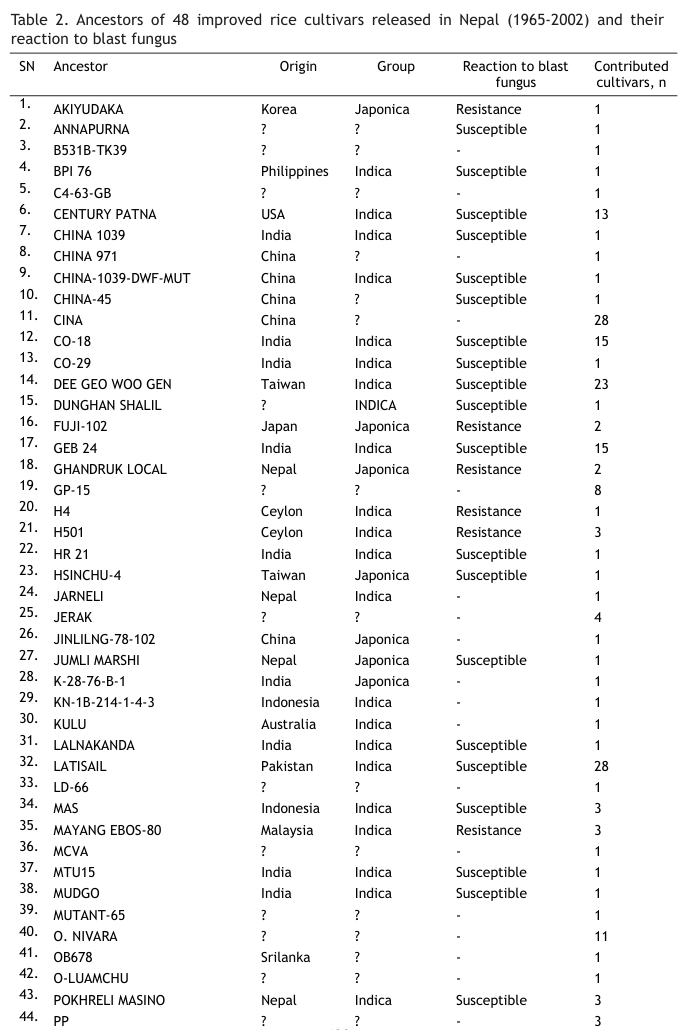
\includegraphics[width=0.75\linewidth]{../images/resistance_breeding_rice_blast_pedigree}

\ecolumns
\end{frame}

\begin{frame}{Marker assisted screening of rice blast resistance}
\protect\hypertarget{marker-assisted-screening-of-rice-blast-resistance}{}
\begin{itemize}
\tightlist
\item
  Refer to the article title ``Screening Nepalese rice germplasm for
  blast resistance characters using molecular markers'' from
  ``Proceedings of Marker Assisted Screening on Cereal in Nepal, 2012''
  (file contained within `literatures/articles').
\end{itemize}
\end{frame}

\begin{frame}{Marker assisted screening of Rice BLB resistance}
\protect\hypertarget{marker-assisted-screening-of-rice-blb-resistance}{}
\footnotesize

\begin{itemize}
\tightlist
\item
  96 Nepalese rice accessions were screened using eight SSR markers and
  one STS marker for presence and absence of BLB resistance genes
  \citep{amgai2015marker}. Resistance gene detected in respective number
  of accessions follows:

  \begin{itemize}
  \scriptsize
  \item Xa-10: 5 accessions
  \item Xa-13: 6 accessions
  \item Xa-7: 23 accessions
  \item Xa-3: 52 accessions
  \item Xa-4: 52 accessions
  \item Xa-5: 25 accessions
  \item Xa-8: 30 accessions
  \item Xa-21: None
  \end{itemize}
\item
  Xa-13 was recovered from susceptible check germplasm, indicating that
  resistance has been overcome by the corresponding virulent strain of
  the bacteria ( \emph{Xanthomonas oryzae} pv. \emph{oryzae}).
\end{itemize}
\end{frame}

\begin{frame}{}
\protect\hypertarget{section-4}{}
\small

\begin{itemize}
\tightlist
\item
  Resistant check IR-64 showed the presence of Xa-5, implying that the
  gene is effective against strains of BLB pathogen during the
  contemporary period.
\item
  Xa-21 gene likely to have originated from \emph{O. longistaminata} and
  integrated into some IRRI developed rice varieties \citep{rao2002dna}.
  Base population of Nepalese variety possibly lack introgressions from
  \emph{O. longistaminata}.
\item
  Interestingly, 17 of the germplasm collections (including Masuli
  variety) possessed three or more genes for BLB resistance.
\end{itemize}
\end{frame}

\begin{frame}{Flood/submergence tolerance}
\protect\hypertarget{floodsubmergence-tolerance}{}
\begin{itemize}
\tightlist
\item
  Refer to the tile ``Identification of flood tolerant genes Sub1A and
  SNORKEL from Nepalese rice gene pool'' from ``Proceedings of Marker
  Assisted Screening on Cereal in Nepal, 2012'' (file contained within
  `literatures/articles').
\end{itemize}
\end{frame}

\begin{frame}{Helminthosporium leaf blight in Wheat}
\protect\hypertarget{helminthosporium-leaf-blight-in-wheat}{}
\begin{itemize}
\tightlist
\item
  Sonalika, BL 1473, and Nepal 297 are early-maturing commercial wheat
  cultivars that are susceptible to HLB
  \citep[\citet{van1998breeding}]{duveiller2004controlling}.
\item
  NL 750, NL 781, and Milan/Shanghai-7 are late-maturing, well-adapted,
  advanced breeding lines with high levels of resistance to HLB
  \citep[\citet{hetzler1991interactions}]{van1998breeding}.
\end{itemize}
\end{frame}

\begin{frame}{Resistance for viral disease}
\protect\hypertarget{resistance-for-viral-disease}{}
\begin{itemize}
\tightlist
\item
  In rice, among the 44 screened germplasm 10 were observed to be
  tolerant while other were moderately to highly susceptible
  \citep{upadhyay1982tetep}.

  \begin{itemize}
  \tightlist
  \item
    IR20, IR 2071-627-1, IR C3707-117 2, IR2797-125, Tetep, IR
    1416-128-5-8 and IR 1905-81-3-1 showed the 0.5\% seedling infection
    rates \(\leadsto\) Highly tolerant.
  \end{itemize}
\end{itemize}
\end{frame}

\begin{frame}{Unwavering legacy of Rampur composite}
\protect\hypertarget{unwavering-legacy-of-rampur-composite}{}
\bcolumns
\column{0.5\textwidth}

\begin{itemize}
\tightlist
\item
  In light of reports of downy mildew disease in Nepal beginning in
  1966, Thai Composite \#1 DMR was introduced and later released as
  Rampur Composite in 1975.
\item
  It was one of the top yielders in variety trials conducted at 10
  locations in 1985 and is resistant to the downy mildew pathogen.
\end{itemize}

\column{0.5\textwidth}

\begin{figure}
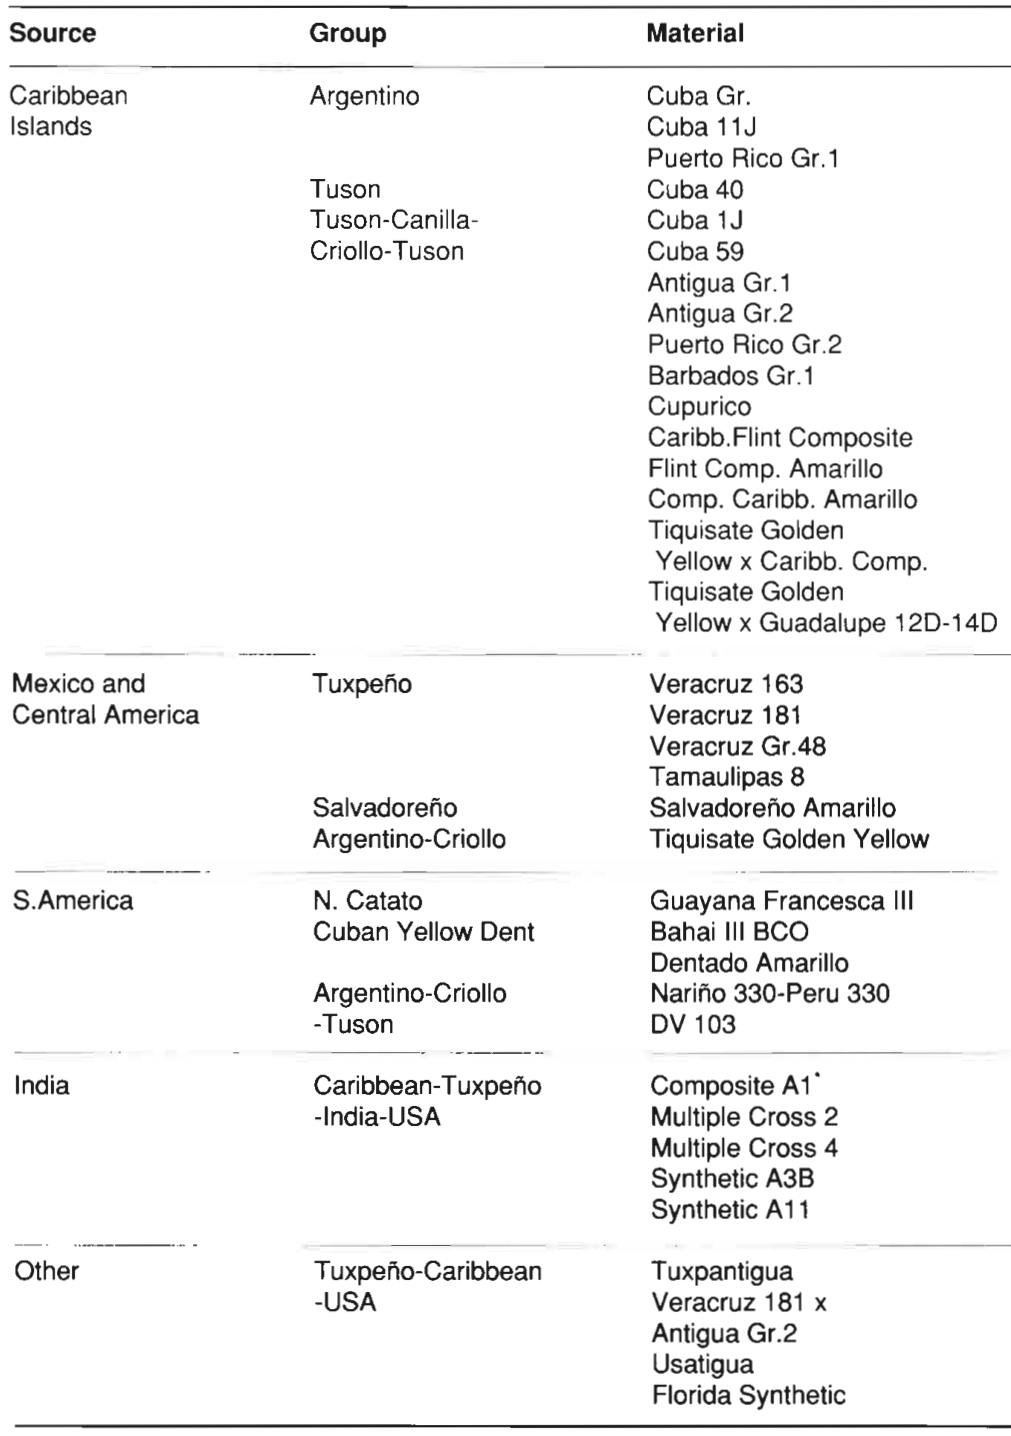
\includegraphics[width=0.4\linewidth]{../images/germplasm_assemblage_thai_composite1} \caption{During the early-to-mid 1960s, staff at Farm Suwan gathered maize varieites and cultivars from around the world. Applying the criteria of known good performance, relative adaptability to Thailand's production conditions, diversity of origin, and useful genetic variability (particularly for traits of economic importance), they finally chose 36 germplasm sources to form a population designated 'Thai Composite \#1'; Source: \cite{sriwatanapongse1993suwan}}\label{fig:thai-composite-germplasm-assembly}
\end{figure}

\ecolumns
\end{frame}

\hypertarget{vegetable-crops}{%
\section{Vegetable Crops}\label{vegetable-crops}}

\begin{frame}{Tomato}
\protect\hypertarget{tomato}{}
\begin{itemize}
\tightlist
\item
  ATY 3, ATY 5, and ATY 6 were resistant to Tomato Yellow Leaf Curl
  Virus (TYLCV) where as NCL1, BL410 and Pusa ruby showed moderate level
  of TYLCV incidence.
\item
  All exotic tomato cultivars are susceptible to leaf curl virus, while
  some local indeterminate cultivars have shown tolerance to Tomato Leaf
  Curl Virus.
\end{itemize}
\end{frame}

\begin{frame}{}
\protect\hypertarget{section-5}{}
\end{frame}

\hypertarget{legumes}{%
\section{Legumes}\label{legumes}}

\begin{frame}{}
\protect\hypertarget{section-6}{}
\begin{itemize}
\tightlist
\item
  Following genotypes (released or under screening) were reported due to
  resistance:

  \begin{itemize}
  \tightlist
  \item
    In soybean, 6 genotypes (PI 94159,G-8754, Dashratpur, SB0095, CM
    9125 and TAMPOMAS) highly resistant to Mungbean Yellow Mosaic Virus
    (MYMV).
  \item
    In mungbean, Pratikshya and Kalyan varieties (released) resistant to
    MYMV.
  \item
    In mungbean, IPM-16 (highly resistant), Hum-12 (resistant) to MYMV
  \item
    In blackgram, Bari Mash-1, Bari Mash-2, Bari Mash-3 (resistant) to
    MYMV
  \end{itemize}
\end{itemize}
\end{frame}

\hypertarget{oil-seed-crops}{%
\section{Oil seed crops}\label{oil-seed-crops}}

\begin{frame}{}
\protect\hypertarget{section-7}{}
\end{frame}

\hypertarget{bibliography}{%
\section{Bibliography}\label{bibliography}}

\begin{frame}{References}
\protect\hypertarget{references}{}
\end{frame}

          \begin{frame}[allowframebreaks]{}
    \bibliographytrue
    \bibliography{./../bibliographies.bib}
    \end{frame}
  


\end{document}
